\title{Tutorial OpenPIV (ver. 0.02)}
\author{
        ver 01: ISTA - Institut f\"ur Str\"omungsmechanik und Technische Akustik\\
        TU - Berlin, \underline{Germany}\\
        ver 02: Turbulence Structure Laboratory, Tel Aviv University, Israel
       }

\date{\today}

%---------- Set-up ------------------------------------------------------
\documentclass[10pt,a4paper]{article}
\usepackage{graphicx,float,url,mathtools}
\usepackage[T1]{fontenc}
\usepackage{listings}
\lstset{%
language=Matlab, 
basicstyle=\footnotesize
}

%---------- Document ----------------------------------------------------
\begin{document}
\maketitle
\tableofcontents
\newpage

%!TEX root=../Tutorial_OpenPIV.tex
\section{Introduction}\label{Intro}

\emph{OpenPIV} is an open source Particle Image Velocimetry (PIV) analysis software written in 
Python, MATLAB and C++. The aim of this document is to deliver a fast overview of the Matlab version of \emph{OpenPIV} only. For Python and C++ see in the respective repositories.
 
The next sections will refer to the main parameters, the output files and other features 
of \emph{OpenPIV}. Some basics of the PIV technique will be mentioned as well. All the distributions  of \emph{OpenPIV} and other related material can be found at \cite{Liberzon:2009,Taylor:2010}.


This tutorial runs \emph{OpenPIV} on MATLAB, nevertheless similar set of parameters and output files applies for other distributions  of \emph{OpenPIV}. The PIV-Data used as example in this tutorial was extracted from \cite{carlier_2005}.

\section{Graphical User Interface GUI}\label{GUI}

The Matlab version of OpenPIV has a graphical user interface (GUI). The program starts from the command window using:



\begin{lstlisting}
	 openpivgui
\end{lstlisting}



The following window is opened:
\begin{figure}[H]
	\centering
	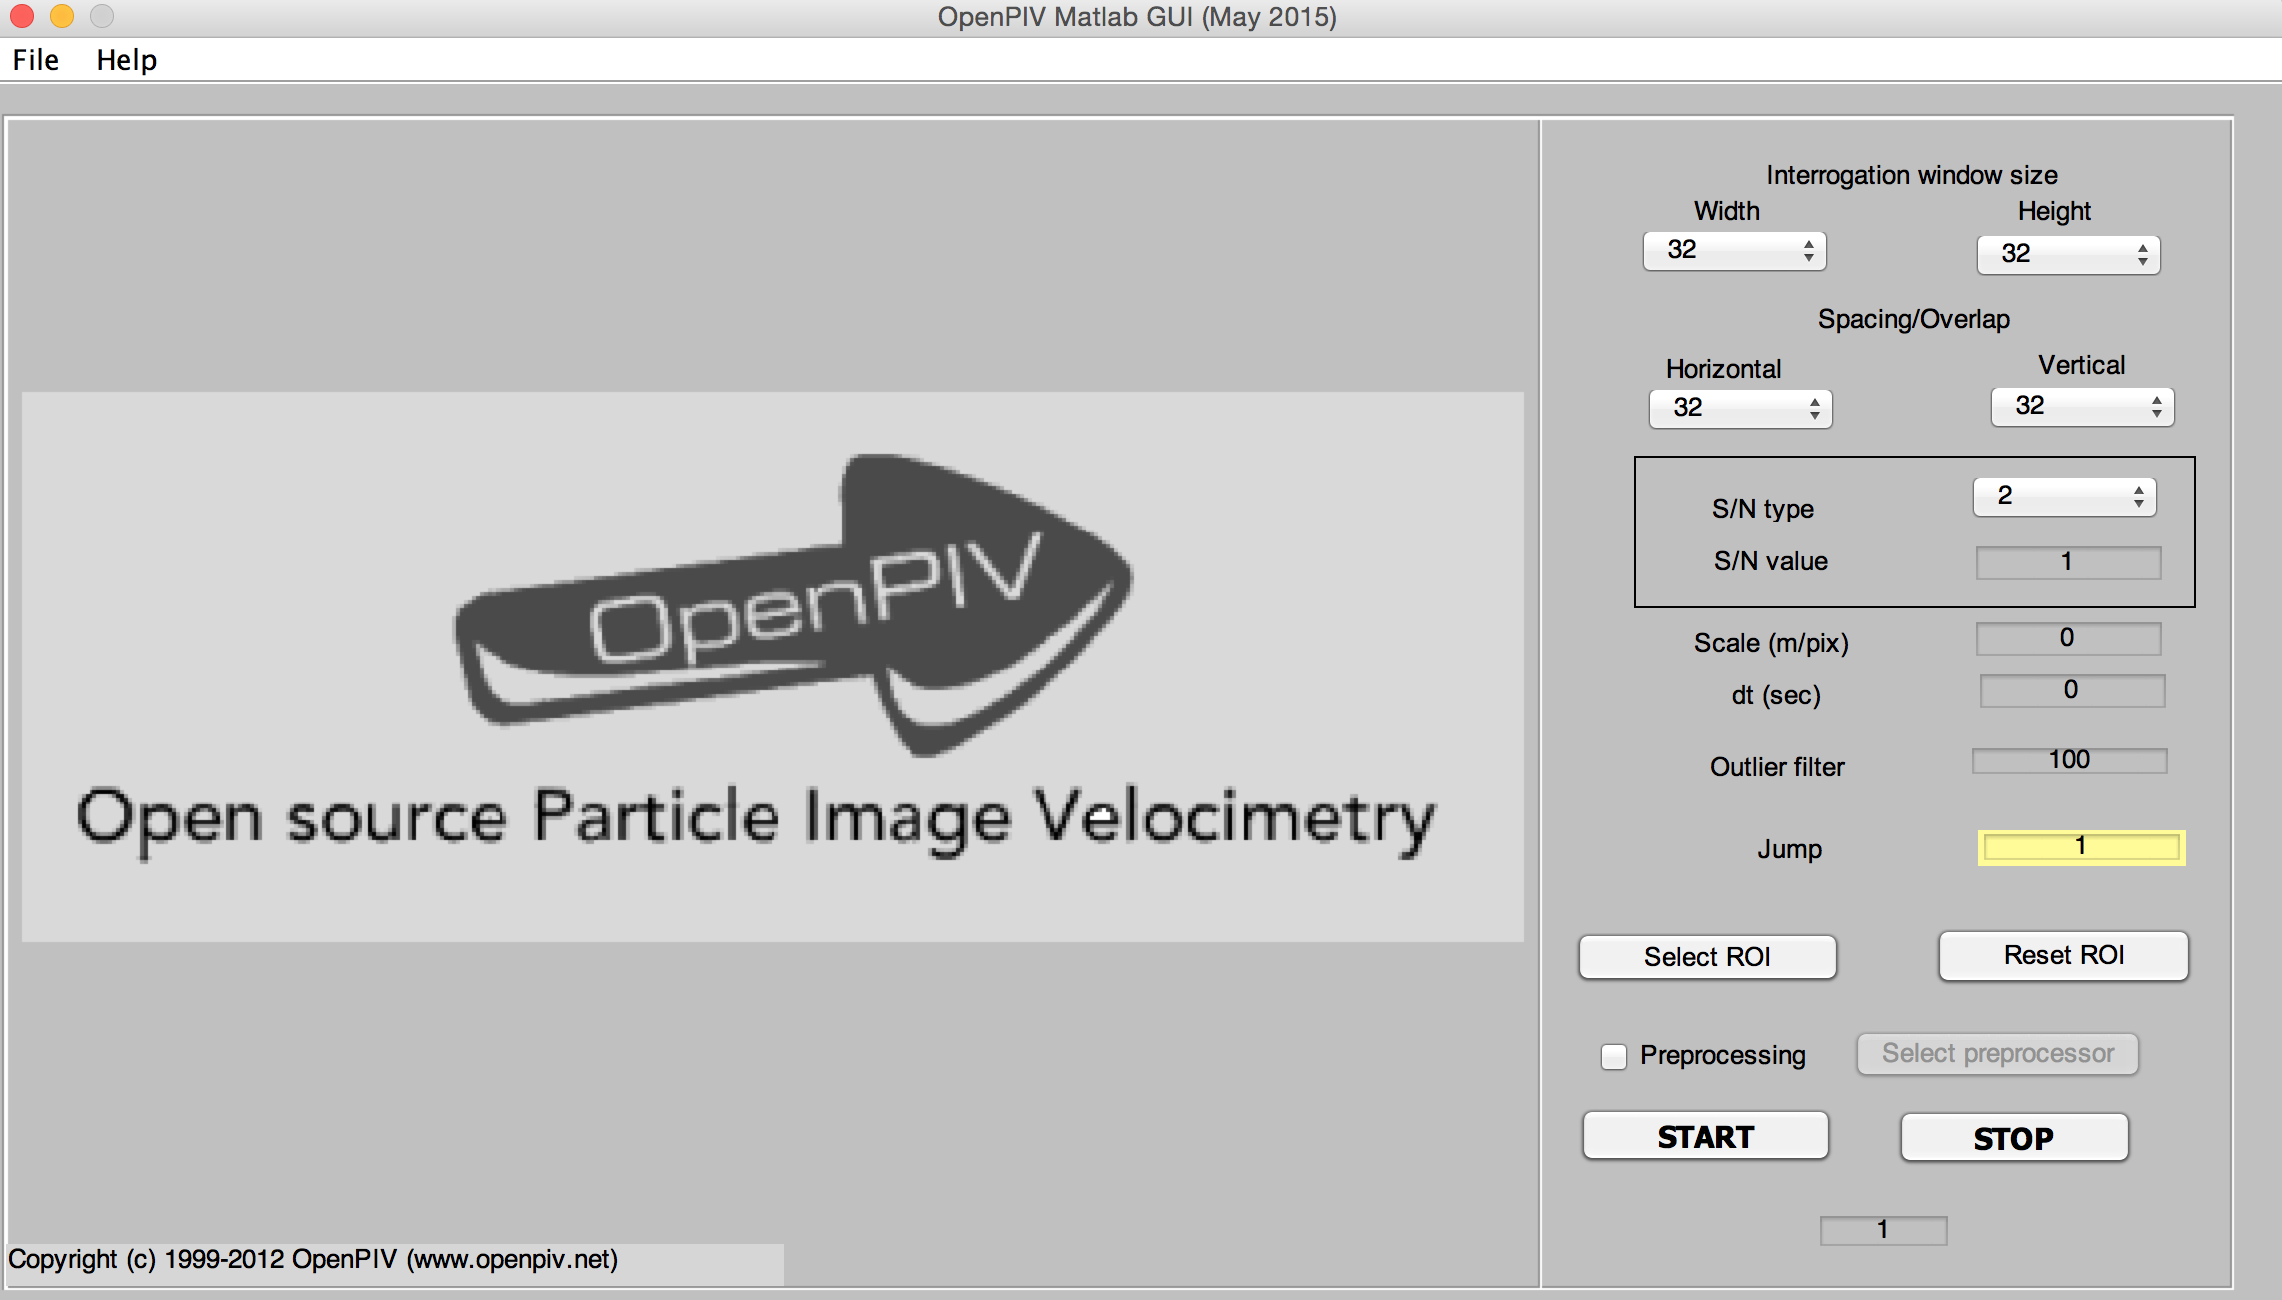
\includegraphics[width=\textwidth]{Images/open_window.png}
	\caption{First window of the OpenPIV}
	\label{fig:open_window}
\end{figure}

Figure \ref{fig:GUI} depicts the Graphical User Interface (GUI) of \emph{OpenPIV} after loading 
some example data.

The first step before to run the PIV-Analysis is to load the PIV-Data. On the top left the menu bar  is located. Under the drop-down menu ``File" the option ``Load" is available, either this option or  its shortcut Ctrl+L opens a window where to select the data to be loaded. Once the PIV-Images are  loaded the buttons $\ll$ and $\gg$ at the bottom jump between the loaded images, the indicator at  the right-bottom displays the number of the currently shown image. 


\begin{figure}[H]
	\centering
	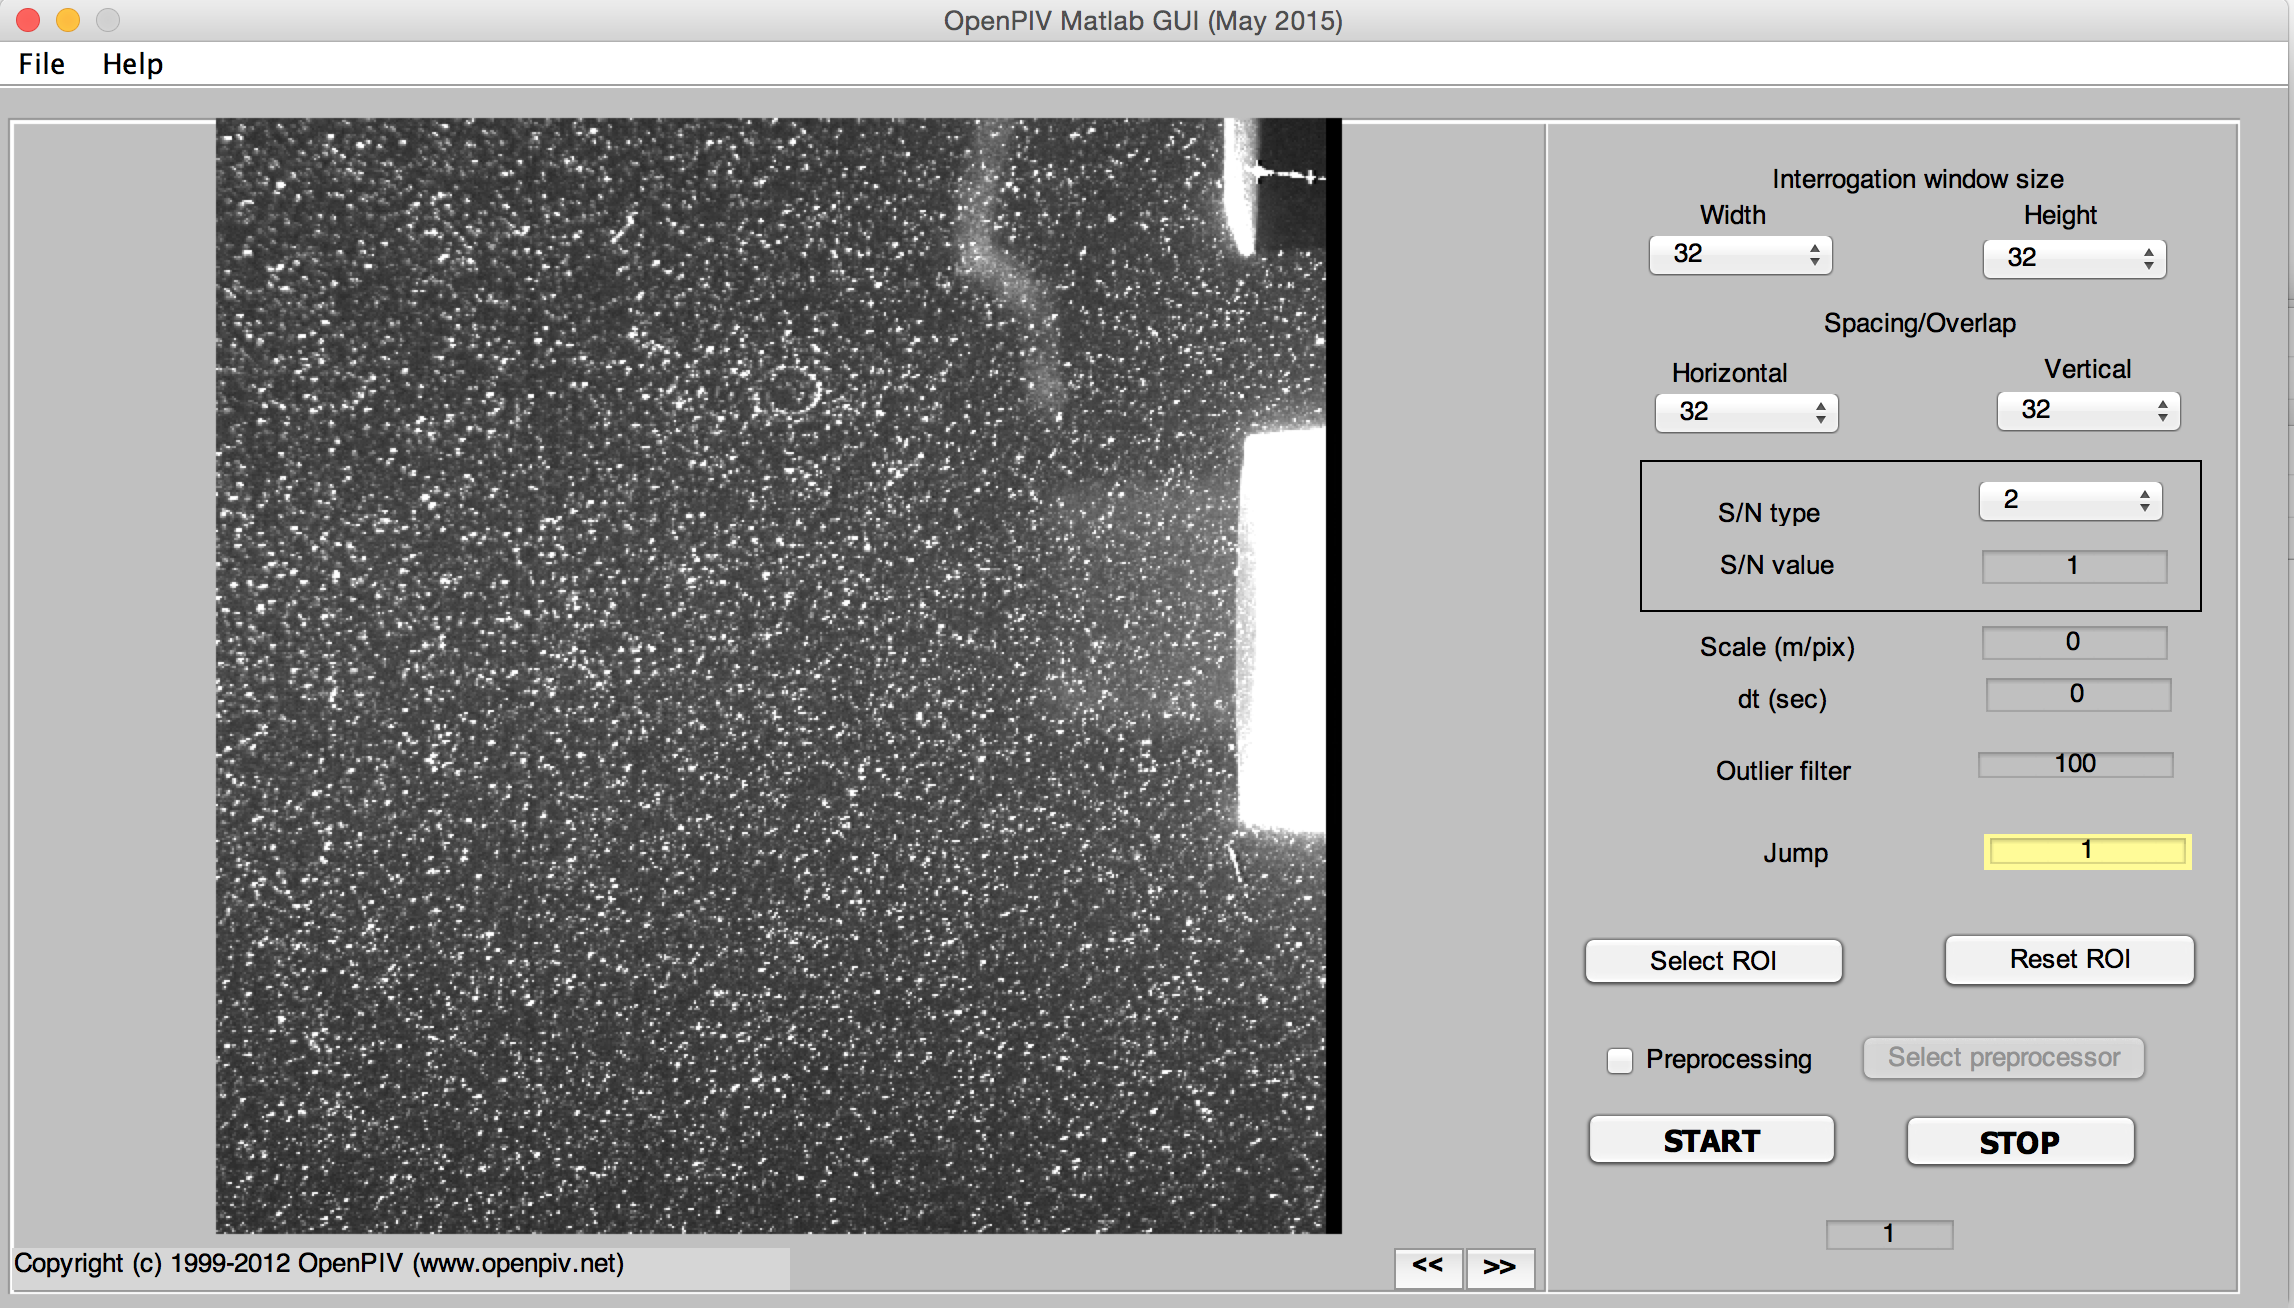
\includegraphics[width=\textwidth]{Images/User_Interface.png}
	\caption{OpenPIV Matlab GUI}
	\label{fig:GUI}
\end{figure}

\section{Load Data}\label{Load}

Note that at least two PIV-Images are needed for a PIV-Analysis. 

\section{Analysis parameters}\label{parameters}
In this section the parameters on the right side of the GUI are described.

\begin{figure}[H]
	\centering
	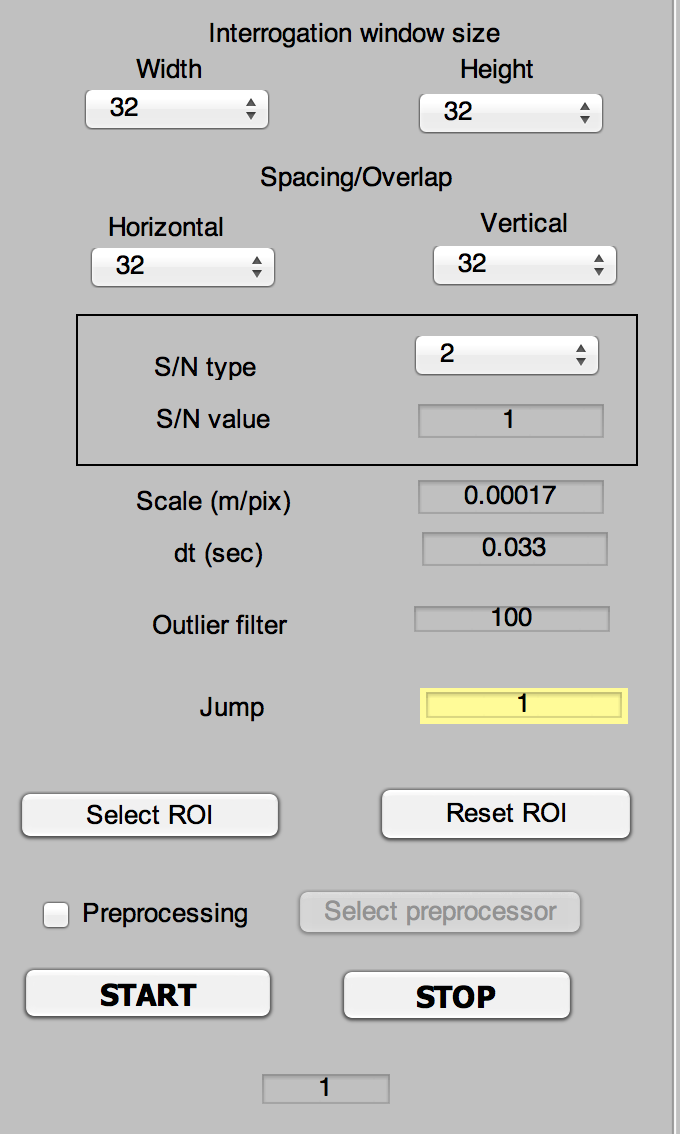
\includegraphics[width=.35\textwidth]{Images/parameters.png}
	\caption{OpenPIV Matlab GUI}
	\label{fig:GUI}
\end{figure}

\subsection{Interrogation window size}\label{Interrogation_Window}
The PIV-Image will be divided in interrogation windows. The width and the height control the size 
in pixels of the interrogation windows. Since the analysis is based on statistical a large 
interrogation windows are more robust against background noise and outlier vectors.

\subsection{Spacing/Overlap}\label{Spacing}
The horizontal and vertical parameters control the size of the correlation windows and set the 
resolution of the two components of the velocity field $u_{x}$ $u_{y}$. In figure \ref{fig:Iwindow} 
is depicted an example.

\begin{figure}[H]
	\centering
	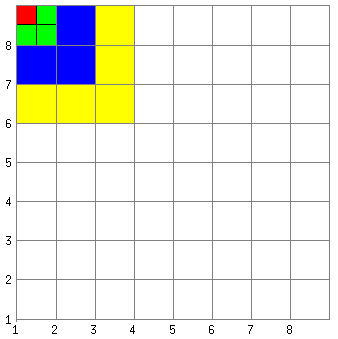
\includegraphics[width=0.4\textwidth]{Images/IntWindow.png}
	\caption{Image of 256x256 pixels divided by 32x32 interrogation window. Space/Overlap: 
                 red 16x16, green 32x32, blue 64x64 and yellow 128x128}
	\label{fig:Iwindow}
\end{figure}

\subsection{Signal-to-Noise ratio and filters}\label{S/N}
In \emph{OpenPIV} are implemented two types of Signal-to-Noise ratio (S/N): \textbf{peak to the mean} and 
\textbf{peak to the second peak}. In the drop-down menu 1 corresponds to peak to the mean and 2 to peak 
to the second peak, option 1 is faster. 


The parameter S/N value is the threshold between the correct/wrong vectors according to the S/N  type. There are no default values, a try-out has to be perform in order to find out the best 
value. 


\emph{OpenPIV} applies global and local filtering. By global filtering the obvious outlier vectors 
will be  removed, i.e. the vectors which length is \textbf{larger than the mean of the flow 
field plus 3 times its standard deviation}. These are global outliers in the statistical sense. 


In order to find local vector outliers, i.e. vectors that are dissimilar from the close neighbors, 
a local filtering is performed on small neighborhoods of vectors, $3 \times 3$. Typically 
there are about 5 \% of erroneous vectors, these are removed and later the missing 
values are interpolated from the neighbor vector values. 

\subsection{Scale}\label{Scale}

The scale value is a factor that will multiply the resulting vectors and the distances between the vectors. It helps with the  visualization of the vectors but it has to be taken into account when the units are transform  to physical units. if the value is null, the scaling is not used. The results will be in pixels. 

\subsection{Time interval}\label{dt}

The time interval is a factor that will convert the displacement (in pixels or meters, if scale is applied) to the speed units (m/sec). the resulting vectors and the distances between the vectors. It helps with the  visualization of the vectors but it has to be taken into account when the units are transform  to physical units. If the value is null, then dt = 1 and the speed will remain as displacement, e.g. pix/dt

\subsection{Outlier filter}\label{Outlier}

The outlier filter value is the threshold of the global outlier filter and indicates \textbf{how many times  the standard deviation of the whole vector field} is exceeded before the vector is considered as  outlier.

\subsection{Jump}\label{Jump}

The jump value indicates how many PIV-Images are evaluated in the analysis. The count starts at 
the next image from the current one, i.e. if jump is equal to \emph{n} then \emph{OpenPIV} takes 
the current image plus the next \emph{n} PIV-Images for one analysis. Note that at least two 
PIV-Images are needed for the analysis, what makes jump values less than one pointless.

\subsection{Select and reset Region Of Interest(ROI)}\label{ROI}
The option Select ROI provides the possibility of evaluate only part of the whole PIV-Image. The 
option Reset ROI release the selected region. In figure \ref{fig:ROI} one example is shown.

\begin{figure}[H]
	\centering
	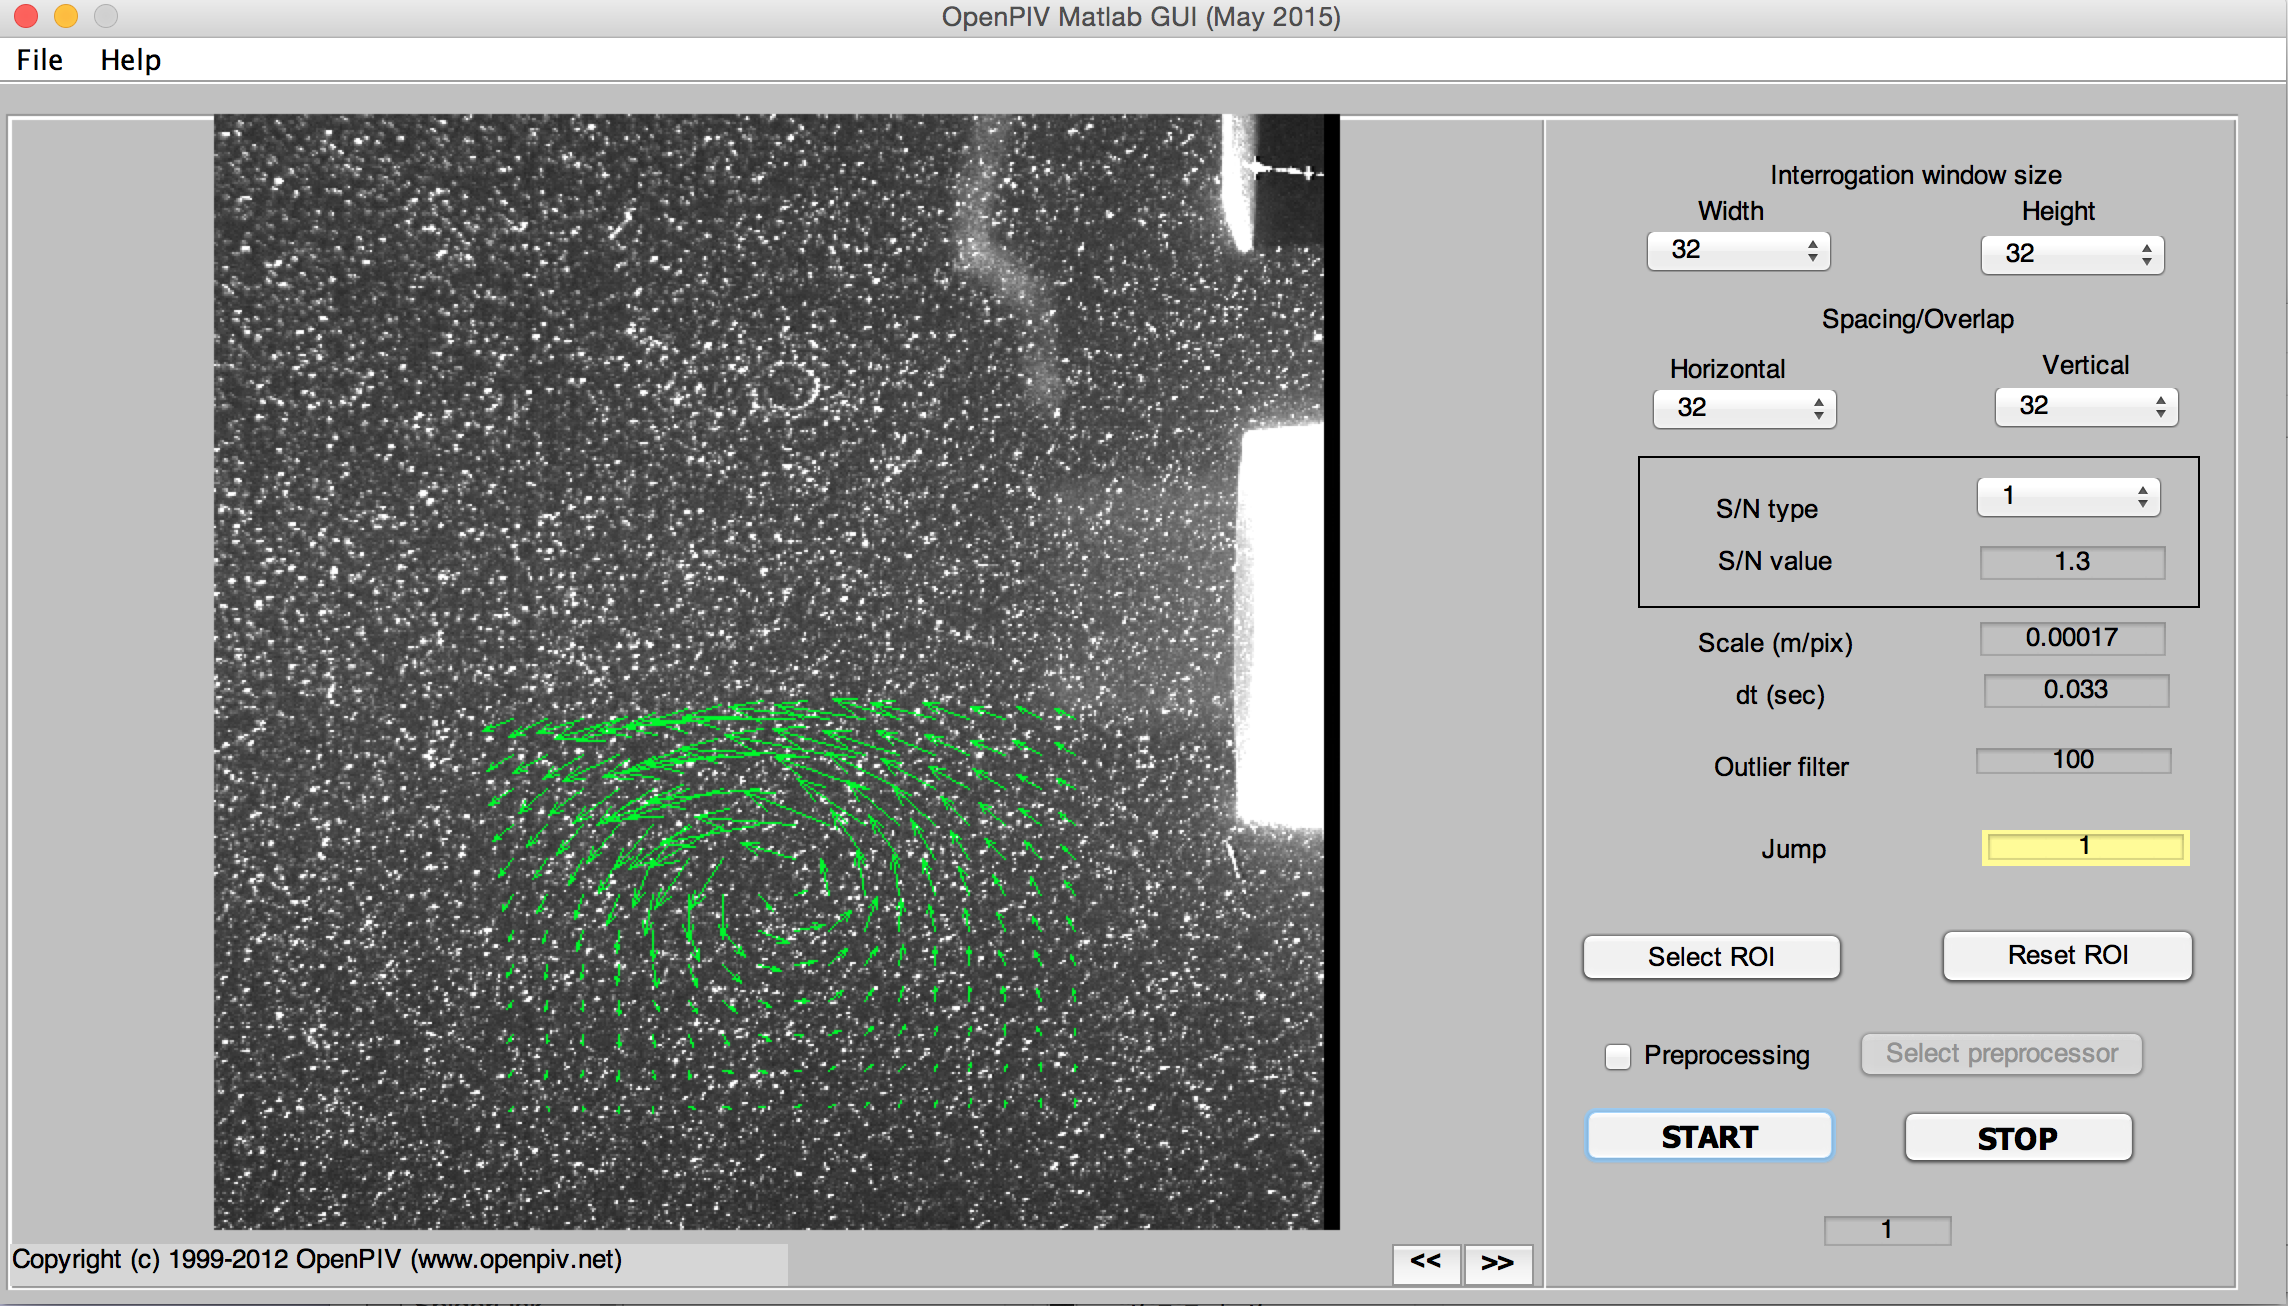
\includegraphics[width=\textwidth]{Images/ROI.png}
	\caption{Results for a selected region}
	\label{fig:ROI}
\end{figure}

\subsection{Pre-processing}\label{Preprocessing}
The pre-processing option applies transformation-image function to the PIV-Images. The current  MATLAB version uses the function \emph{adapthisteq} which enhances the contrast of images.  For more details see MATLAB help. The user can develop any image processing algorithm to run on each of the images before the FFT-based cross-correlation algorithm is applied to get PIV data. 

\section{Start and stop}\label{Start}
The start and stop buttons either start or stop the analyze process.

\section{Output files}\label{Output files}

The first vectors results are depicted on the PIV-Images in the GUI, as figure \ref{fig:ROI} and 
\ref{fig:Out} illustrate. In the folder containing the PIV-Data \emph{OpenPIV} saves three lists 
of files: no filtered results \emph{dataName\_noflt.vec}, filtered results after global and local 
filters \emph{dataName\_flt.vec} and final results after filtering and interpolation 
\emph{dataName.vec}. 

The output file has a \textbf{header} that defines the variables and the units of the \textbf{5 columns} of data, i.e. $x$ $y$ $u_{x}$ $u_{y}$ $S/N$, and the size of the PIV field. 



 \begin{lstlisting}
VARIABLES= "X m", "Y m", "U m/s", "V m/s", "CHC", ZONE I=32, J=32
 \end{lstlisting}
  
  
 Possible units are `pix' or `m' and the velocity can be `pix/dt' or `m/s' (or `pix/s'). The first two columns  correspond to the coordinates, the third and fourth to the two velocity vector components  and the fifth column is the S/N ration. Note that the value is different if the user chose peak  to second peak or peak to mean ratio as S/N type. The value of peak to second peak or peak  to mean ratio is stored for further processing.



The number of output files will be the number of loaded PIV-Images minus the selected jump value.
\begin{figure}[H]
	\centering
	\includegraphics[width=\textwidth]{Images/output.png}
	\caption{Output results}
	\label{fig:Out}
\end{figure}


\clearpage
\appendix
\section*{Appendix: Units convert}\label{Units}

Sometimes it makes more sense to leave the scale and time interval as default and transform the units of the results manually. In this case the velocity vector units of $u_{x}$ and $u_{y}$ are stored as displacements. \emph{OpenPIV} results are delivered in $[scale\times(pixels/\Delta t)]$, 
with $scale$ as the selected scale value and $\Delta t$ as the time interval between two images. 
In order to convert the units to $[m/s]$ is needed:

\begin{itemize}
      	\item the vector components $u_{x}$, $u_{y}$ in $[scale\times(pixels/\Delta t)]$
      	\item the $\Delta t$ value in $s$
      	\item the dimensionless scale value
	\item the relation between $meters$ and $pixels$ in that image $[m/pixels]$, i.e. the 
	      image size and the number of pixels.
\end{itemize}

The following example demonstrates a particular case of unit conversion.

\begin{itemize}
      	\item $u_{x}$ = 5, $u_{y}$ = 0 in $[scale\times(pixels/\Delta t)]$
      	\item the $\Delta t$ = 0.5 in $s$
      	\item scale value = 2
        \item image size 0.25 x 0.25 $m$ and 256 x 256 $pixels$, i.e. the relation between 
	      $meters$ and $pixels$ is 0.25/256 $[m/pixels]$.
    	\item the conversion of $u_{x}$ from $[scale\times(pixels/\Delta t)]$ to $[m/s]$:
        \[
         \frac{u_{x}}{scale\times\Delta t}\times rel.\frac{m}{pixels}=\frac{5}{2\times0.5}\times 
         \frac{0.25}{256}=0.0049 m/s
        \]
\end{itemize}


%---------- Bibliography ------------------------------------------------
\bibliographystyle{unsrt}       % this means that the order of references
                                % is dtermined by the order in which the
                              	% \cite and \nocite commands appear
\bibliography{PIVbib}	      	% list here all the bibliographies that
%                           	% you need.
\end{document}
